\documentclass[11pt,a4paper]{article}
\usepackage[margin=1in]{geometry}
\usepackage{hyperref}
\usepackage{enumitem}
\usepackage{graphicx}
\usepackage{xcolor}

% Added for this proposal: tables and vector diagrams.
\usepackage{booktabs}
\usepackage{tabularx}
\usepackage{tikz}
\usetikzlibrary{arrows.meta,positioning,fit,calc}

% -----------------------------------------------------
% bvraghav-tiet-ucs503p-article.sty
% -----------------------------------------------------

% Variable: Lab Instructor
\makeatletter \newcommand{\BvrSetLabInstructor}[1]{%
  \gdef\Bvr@LabInstructor{#1}}
% default
\newcommand{\Bvr@LabInstructor}{Ms. Paramveer Sidhu}
% public accessor
\newcommand{\BvrLabInstructorValue}{\Bvr@LabInstructor}
\makeatother

% Add subtitle
\usepackage{titling}
% -- Set title bold
\pretitle{\begin{center}\bfseries\fontsize{18bp}{18bp}\selectfont}
\makeatletter
\newcommand{\BvrSubtitle}[1]{%
  \posttitle{%
    \par\end{center}
    \begin{center}\large#1\end{center}
    \vskip 0.5em}%
}
\makeatother

% Hints in the section title(s)
\newcommand{\BvrHint}[1]{%
  {\normalfont\normalsize\itshape\hfill #1}}

% -----------------------------------------------------

% Diagram palette (kept muted for print)
\definecolor{teAccent}{HTML}{1F4E79}
\definecolor{teFill}{HTML}{EAF1F8}
\definecolor{teExt}{HTML}{F5EFE3}
\definecolor{teExtLine}{HTML}{8A6D3B}

\hypersetup{
  colorlinks=true,
  linkcolor=teAccent,
  urlcolor=teAccent,
  citecolor=teAccent,
  pdftitle={TripEase: An Integrated Trip Planning and Itinerary Management System},
  pdfsubject={UCS503P Project Proposal}
}

\title{TripEase: An Integrated Trip Planning and
  Itinerary Management System}

\BvrSetLabInstructor{Ms. Paramveer Sidhu}

\BvrSubtitle{%
  Project Proposal for UCS503P  \\
  Submitted to: \BvrLabInstructorValue \\ \bfseries
  Thapar Institute of Engineering and Technology%
}

% -----------------------------------------------------

\author{
  Manraj Singh, COE%
  \thanks{Roll No: \texttt{1024030712}, %
    Email: \texttt{msingh17\_be24@thapar.edu}}
  \and
  Vatsal Chauhan, COE%
  \thanks{Roll No: \texttt{1024030714}, %
    Email: \texttt{vchauhan\_be24@thapar.edu}}
  \and
  Nimitt Malhotra, COE%
  \thanks{Roll No: \texttt{1024030709}, %
    Email: \texttt{nmalhotra\_be24@thapar.edu}}
}

\date{\today}

\begin{document}
\maketitle

\section{Higher-order goal%
  \BvrHint{\ldots secondary framing}}
Planning a shared trip is a coordination problem before
it is a travel problem. A group agrees on a
destination, then spends days re-deciding the same
questions --- what are we seeing on Tuesday, who paid
for the cab, is the fort before or after lunch ---
because the answers live in five different apps and
nobody owns the current version.

The broader goal we are framing this project against is
\emph{reducing coordination overhead in small-group
  decision making}. That is deliberately larger than
one web application, and we are not claiming to solve
it. The immediate engineering objective is narrower and
testable: give a small group one shared, editable
artefact --- a trip --- that holds the plan, the
geography and the money together, and measure whether
producing that artefact takes materially less effort
than the current do-it-yourself workflow.

A modest secondary benefit is that a plan with real
route information attached tends to be a less wasteful
plan. Groups that can see their day laid out on a map
avoid the backtracking that comes from ordering stops
by memory. We mention this as framing only; it is not
something we intend to measure in this course.

\section{Time-to-value %
\BvrHint{\ldots primary heuristic}}
\begin{itemize}[leftmargin=0.7cm]
    \item The first shippable increment is a
      \emph{thin vertical slice}: sign in, create a
      trip, add named places to it, see it again on
      reload. It touches authentication, the data
      model, the UI shell and the deployment pipeline,
      so it de-risks all four at once instead of
      building any one of them to completion.
    \item We work in one-week iterations, with a
      demonstrable increment deployed to a staging URL
      at the end of each. Feedback is collected from
      real classmates planning real trips, not from
      ourselves.
    \item CI is set up in iteration~1, before the
      feature work grows. Every push runs lint, unit
      tests and a production build; merges to
      \texttt{master} deploy to staging automatically.
      The cost of doing this early is roughly a day;
      the cost of retrofitting it in week~six is much
      higher.
    \item We prefer a narrow feature that is deployed
      over a broad feature that is half-written on a
      branch. Where the two conflict, scope is cut, not
      the release.
\end{itemize}

\section{Problem Statement}
Trip planning is not blocked by a lack of tools. It is
blocked by the fact that the tools do not share state.
A student group at this institute planning a four-day
trip to Jaipur or Manali will typically end up using:
a search engine and travel blogs for deciding what is
worth seeing; Google Maps for checking whether two
places are anywhere near each other; a notes app or a
shared document for the day-by-day plan; a spreadsheet
for the budget and for who owes whom; and a WhatsApp
group where all of the above get pasted, discussed and
then lost in the scrollback.

The observable pain points are:

\begin{itemize}[leftmargin=0.7cm]
    \item \textbf{No single source of truth.} The
      itinerary exists in three places at once and they
      disagree. The most recent version is whichever
      one the loudest person is reading from.
    \item \textbf{Geography is disconnected from the
      plan.} The day order is decided in a text
      document, where nothing warns you that stop~2 and
      stop~3 are on opposite sides of the city. The
      mismatch is discovered on the road.
    \item \textbf{Manual, repeated arithmetic.}
      Budgets are re-totalled by hand every time
      something changes, and expense splitting is done
      after the trip from memory and screenshots.
    \item \textbf{Sharing is lossy.} Sending the plan
      to someone means exporting it into a message,
      after which their copy immediately goes stale.
    \item \textbf{Re-work.} None of the effort is
      reusable. The next trip starts from an empty
      document again.
\end{itemize}

\textbf{Contextual relevance.} The stakeholders here
are our immediate peers. Group trips planned over a
weekend by five or six students, on mid-range Android
phones, on hostel Wi-Fi, are a workload we can observe
directly and get feedback on within a single iteration.
We are not designing for a travel agency.

\textbf{Formal statement.} \emph{Design and build a
  web-based system that lets a user assemble a
  multi-day trip --- destinations, an ordered day-wise
  itinerary, the route between stops, and a categorised
  budget with actual expenses --- as a single persistent
  shared record, and that reduces the time and the
  number of separate tools required to produce a
  complete, agreed itinerary.}

\section{Proposed Solution %
\BvrHint{\ldots Software Proposition}}

\subsection{Overview}
TripEase is a responsive web application in which a
\emph{trip} is the central object and everything else
hangs off it.

\begin{itemize}[leftmargin=0.7cm]
    \item \textbf{Accounts and trips:} email/password
      and Google sign-in; a dashboard listing the
      user's trips; create, rename, edit dates and
      delete.
    \item \textbf{Place capture:} search for a place by
      name using an autocomplete backed by a maps
      provider, and attach it to the trip with its
      coordinates and identifier resolved.
    \item \textbf{Day-wise itinerary:} assign captured
      places to days and order them within a day.
      Reordering is a drag or an up/down control, not a
      re-typed document.
    \item \textbf{Map and route view:} the selected
      day's stops drawn as ordered markers with a route
      polyline, plus leg distance and travel time, so
      the plan is checked against geography while it is
      being made rather than afterwards.
    \item \textbf{Budget and expenses:} a planned
      budget split by category, actual expenses logged
      against those categories, and a running
      planned-versus-actual total.
    \item \textbf{Sharing:} a read-only link to the
      current itinerary, so the shared copy stays live
      instead of being a stale paste.
\end{itemize}

\subsection{Core workflow}
\begin{enumerate}[leftmargin=0.7cm]
    \item User signs in and creates a trip with a
      destination and a date range. The number of days
      follows from the dates.
    \item User searches for places and adds them to the
      trip's place list.
    \item User assigns places to days and orders them.
    \item The map view draws the day's route and
      reports leg distances and durations; the user
      adjusts the order if it looks wrong.
    \item User sets a budget per category and logs
      expenses as they occur.
    \item User shares a read-only link with the rest of
      the group.
\end{enumerate}

Figure~\ref{fig:workflow} shows this as a flow. Every
step after sign-in writes to the same trip document, so
there is only ever one current version of the plan.

\begin{figure}[htbp]
\centering
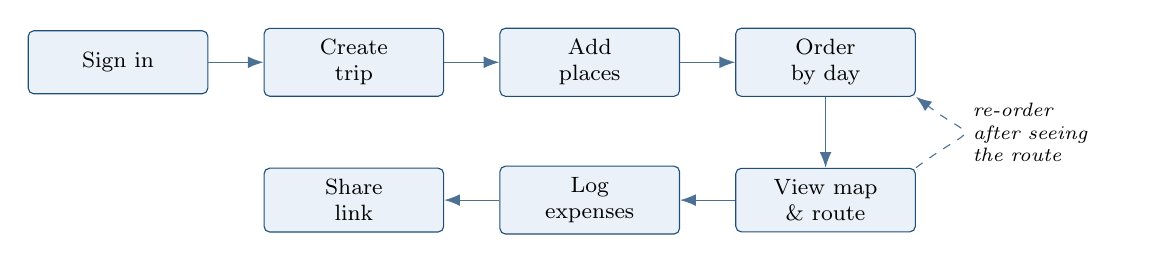
\begin{tikzpicture}[
  node distance=6mm and 7mm,
  box/.style={draw=teAccent,fill=teFill,rounded corners=2pt,
    align=center,inner sep=4pt,font=\footnotesize,
    minimum height=8mm,text width=20mm},
  ar/.style={-{Latex[length=2mm]},draw=teAccent!80}
]
\node[box] (a) {Sign in};
\node[box,right=of a] (b) {Create\\trip};
\node[box,right=of b] (c) {Add\\places};
\node[box,right=of c] (d) {Order\\by day};
\node[box,below=9mm of d] (e) {View map\\ \& route};
\node[box,left=of e] (f) {Log\\expenses};
\node[box,left=of f] (g) {Share\\link};
\draw[ar] (a)--(b); \draw[ar] (b)--(c); \draw[ar] (c)--(d);
\draw[ar] (d)--(e); \draw[ar] (e)--(f); \draw[ar] (f)--(g);
\draw[ar,dashed] (e.north east) .. controls +(8mm,6mm) and +(8mm,-6mm) .. (d.south east)
  node[midway,right,font=\scriptsize\itshape,text width=19mm,align=left]
  {re-order\\after seeing\\the route};
\end{tikzpicture}
\caption{Proposed core workflow. The dashed edge is the
  feedback loop that the current do-it-yourself
  workflow lacks: the plan is checked against real
  geography while it is being written.}
\label{fig:workflow}
\end{figure}

\subsection{What this is not}
To keep the scope honest: TripEase does not book
anything, does not price flights or hotels, and does
not generate itineraries automatically. Those are
discussed in \S\ref{sec:scope} as later or
out-of-course work. The first release is a planning and
record-keeping tool.

\subsection{Operational constraints}
\begin{itemize}[leftmargin=0.7cm]
    \item Mobile-first responsive layout. Planning
      happens on phones; the map view must be usable on
      a small screen, not merely render on one.
    \item Tolerant of poor connectivity: reads are
      cached where the client library allows it, and a
      failed map call degrades to the list view rather
      than blanking the page.
    \item No dependence on unpublished or research-grade
      algorithms. Ordering aids are heuristic and always
      overridable by the user.
\end{itemize}

\section{Solution Approach %
\BvrHint{\ldots Engineering focus}}
This is an engineering course project. The interesting
work is in the data model, the access rules, the
integration boundaries and the release process --- not
in inventing new algorithms.

\subsection{Architecture %
\BvrHint{\ldots web-based solution}}
We propose a client-centric architecture over managed
backend services rather than a hand-written server
tier, as shown in Figure~\ref{fig:arch}.

\begin{figure}[htbp]
\centering
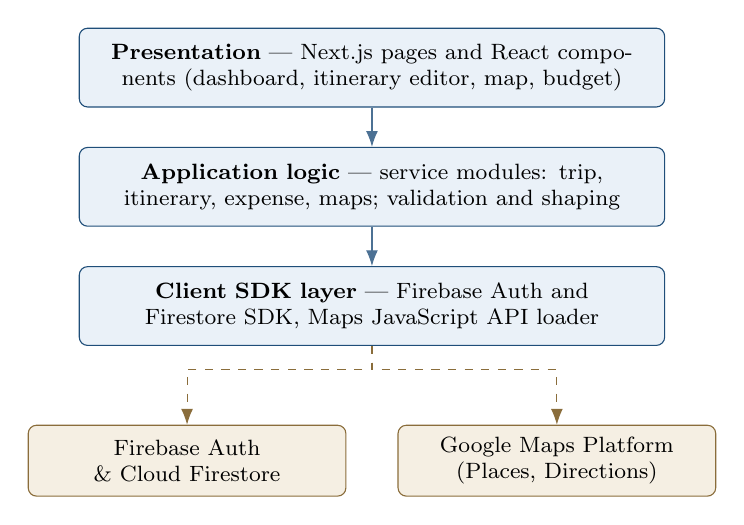
\begin{tikzpicture}[
  node distance=5mm,
  layer/.style={draw=teAccent,fill=teFill,rounded corners=3pt,
    align=center,font=\footnotesize,minimum height=10mm,text width=72mm},
  ext/.style={draw=teExtLine,fill=teExt,rounded corners=3pt,
    align=center,font=\footnotesize,minimum height=9mm,text width=38mm},
  ar/.style={-{Latex[length=2mm]},draw=teAccent!80},
  arx/.style={-{Latex[length=2mm]},draw=teExtLine,dashed}
]
\node[layer] (ui) {\textbf{Presentation} --- Next.js pages and React
  components (dashboard, itinerary editor, map, budget)};
\node[layer,below=of ui] (app) {\textbf{Application logic} --- service modules:
  trip, itinerary, expense, maps; validation and shaping};
\node[layer,below=of app] (sdk) {\textbf{Client SDK layer} --- Firebase Auth
  and Firestore SDK, Maps JavaScript API loader};

\node[ext,below left=10mm and -34mm of sdk] (fb) {Firebase Auth\\ \& Cloud Firestore};
\node[ext,below right=10mm and -34mm of sdk] (gm) {Google Maps Platform\\ (Places, Directions)};

\draw[ar] (ui)--(app); \draw[ar] (app)--(sdk);
\draw[arx] (sdk.south) -- ++(0,-3mm) -| (fb.north);
\draw[arx] (sdk.south) -- ++(0,-3mm) -| (gm.north);
\node[right=1mm of ui.east,font=\scriptsize\itshape,rotate=90,anchor=south] {};
\end{tikzpicture}
\caption{Proposed architecture. Solid edges are
  in-application calls; dashed edges cross a trust
  boundary into managed third-party services.}
\label{fig:arch}
\end{figure}

\textbf{Why no separate backend server?} A conventional
three-tier design would mean writing, hosting,
securing and monitoring an API server whose only real
job would be to forward CRUD operations to a database.
For a three-person team on a one-semester schedule that
is overhead without a corresponding benefit. Firebase
Authentication and Firestore provide identity and
persistence directly, and Firestore security rules move
authorisation into a declarative, testable artefact
that lives in the repository. The trade-off we accept
is vendor lock-in and less control over query planning;
we consider that acceptable at this scale, and the
service modules in the application layer exist
specifically so that data access is not scattered
through the components if it ever has to change.

We do expect to need a small amount of server-side
code, and Next.js route handlers cover it without a
separate deployment: the Directions call and the
read-only share endpoint should run server-side so the
corresponding API key is never shipped to the browser.

\subsection{Maps integration %
\BvrHint{\ldots planned, not connected}}
Three distinct capabilities are involved, and it is
worth separating them because they have different cost
and caching characteristics:

\begin{itemize}[leftmargin=0.7cm]
    \item \textbf{Places / Autocomplete} --- turning
      what the user typed into a specific place with a
      stable identifier and coordinates.
    \item \textbf{Geocoding} --- address or place name
      to latitude/longitude, and the reverse where a
      user drops a pin.
    \item \textbf{Directions} --- an ordered list of
      stops to a route, with per-leg distance and
      duration.
\end{itemize}

Maps Platform terms restrict how long most place
content may be stored, while place identifiers may be
retained. Our data model therefore stores the
identifier, the coordinates and a user-visible label,
and re-fetches presentation details on demand. This is
a real constraint on the schema, not a footnote, and we
have designed around it rather than discovering it
later.

\subsection{Ordering aid %
\BvrHint{\ldots non-research}}
Suggesting a sensible order for a day's stops is a
travelling-salesman variant. We are explicitly not
solving it. For the five-to-eight stops a real day
contains, we apply a nearest-neighbour pass over
straight-line distances and present it as a suggestion
the user may accept or ignore. The user's manual order
always wins, and the suggestion is never applied
silently. We will not claim optimality.

\subsection{CI/CD}
\begin{itemize}[leftmargin=0.7cm]
    \item GitHub Actions runs lint, unit tests and a
      production build on every push and pull request.
    \item Firestore security rules are tested in CI
      against the emulator, so an authorisation
      regression fails the build rather than reaching
      staging.
    \item Merges to \texttt{master} deploy to a staging
      environment with its own Firebase project, so
      pilot data never mixes with development data.
    \item Secrets live in repository secrets and in
      \texttt{.env.local}; \texttt{.env.example} is
      committed, real keys are not.
\end{itemize}

\section{Evaluation Criterion %
\BvrHint{\ldots measurable and attributable}}
All figures below are \textbf{pre-registered targets}
for the pilot, fixed before development so that they
cannot be adjusted to fit whatever we happen to
observe. They are not results. Nothing has been
measured yet.

\subsection{Primary metric}
\textbf{Time-to-complete-itinerary (TTCI):} elapsed
time from trip creation to the trip reaching a
\emph{complete} state, defined as every day in the
range having at least one ordered stop and a budget
figure recorded.

\begin{itemize}[leftmargin=0.7cm]
    \item \textbf{Target:} median TTCI $\le$ 15 minutes
      for a standardised task --- a 3-day trip with at
      least 5 stops --- for first-time users.
    \item \textbf{Attribution:} computed from server
      timestamps written by the application
      (\texttt{createdAt} on the trip document, and the
      write that first satisfies the completeness
      predicate). It is derived from data the system
      already stores, so it does not depend on
      self-reporting.
    \item \textbf{Baseline:} the same task performed
      with the participant's existing tools, timed by
      observation, collected from the same participants
      before they use TripEase.
\end{itemize}

\subsection{Secondary metrics}
\begin{itemize}[leftmargin=0.7cm]
    \item \textbf{Tool count:} number of distinct
      applications the participant used to complete the
      task, before versus after. Target: reduced to one
      for the planning task itself.
    \item \textbf{Task completion rate:} share of
      participants who reach a complete itinerary
      unaided. Target: $\ge$ 80\%.
    \item \textbf{Re-order rate after route view:} how
      often a user changes a day's order after seeing
      the route. This is our check on whether the map
      is actually informing the plan or is decoration.
    \item \textbf{Perceived clarity:} single 1--5 item
      on whether the itinerary was easy to follow.
      Target: mean $\ge$ 4.
    \item \textbf{Reliability:} sign-in and trip-save
      available on staging during the pilot window.
      Target: $\ge$ 99\%.
    \item \textbf{Delivery cadence:} number of
      iterations that ended with a green build deployed
      to staging. Target: every iteration. This one
      measures our process, not the product, and the
      course criteria make it a first-class metric.
\end{itemize}

\subsection{Pilot plan %
\BvrHint{\ldots high-level}}
\begin{itemize}[leftmargin=0.7cm]
    \item 12--20 participants drawn from classmates who
      have planned a group trip in the last year.
    \item Each performs the standardised task once on
      their existing tools (baseline, observed) and
      once on TripEase, with order counterbalanced
      across participants to blunt the learning effect.
    \item Instrumentation is in the application from
      iteration~2, so the metric is available for every
      iteration and not just at the end.
    \item Participants are told what is being recorded;
      no location history or contact data is collected.
\end{itemize}

\section{Scalability %
\BvrHint{\ldots with foresight}}

\begin{enumerate}[leftmargin=0.7cm]
    \item \textbf{Scalable in principle.} Growth here
      is in trips and concurrent editors, not in
      compute.
    \begin{itemize}[leftmargin=0.7cm]
        \item Trips are a top-level collection keyed by
          owner, with itinerary items and expenses as
          subcollections. Queries stay bounded to a
          single trip; a user with 200 trips loads a
          page of them, not all of them.
        \item Every list query is indexed and paginated
          with cursors, so cost is proportional to what
          is displayed rather than to collection size.
        \item Counters and totals that would otherwise
          require reading a whole subcollection are
          maintained as denormalised fields on the trip
          document, updated in a transaction.
        \item The client is stateless with respect to
          the server; there is no session affinity to
          preserve.
    \end{itemize}

    \item \textbf{Operationally deployable.} The
      deployment story is deliberately boring.
    \begin{itemize}[leftmargin=0.7cm]
        \item Static and server-rendered output hosted
          on a managed platform with a CDN in front.
        \item Managed, replicated datastore; no
          database administration on our side.
        \item Separate development, staging and
          production projects with separate keys and
          quotas.
        \item Deployment is a pipeline job, so a
          release is repeatable and revertible rather
          than a manual sequence someone remembers.
    \end{itemize}
\end{enumerate}

The honest limit is cost, not architecture: Maps
Platform calls are billed per request, so at large
scale the constraint becomes autocomplete session
management and caching what the terms permit, rather
than servers.

\section{Engine availability heuristic}
Every component of the core solution already exists as
a mature, documented product. Table~\ref{tab:engines}
lists them with the reason for each choice.

\begin{table}[htbp]
\centering
\footnotesize
\caption{Engines selected, with rationale. No component
  requires research work.}
\label{tab:engines}
\begin{tabularx}{\textwidth}{@{}l l X@{}}
\toprule
\textbf{Concern} & \textbf{Engine} & \textbf{Why this one} \\
\midrule
UI and routing & Next.js (React) & File-based routing and server
  route handlers let us keep the Directions key server-side without
  operating a second service; one deployable artefact. \\
Identity & Firebase Authentication & Email/password and Google
  sign-in without hand-rolling password storage or session handling
  --- an area where a student implementation is most likely to be
  quietly wrong. \\
Persistence & Cloud Firestore & Document model matches a trip's
  nested, variable-shape structure; live listeners give
  multi-device consistency for free, which is the basis for later
  collaborative editing. \\
Geography & Google Maps Platform & Places, Geocoding and Directions
  from one provider with a single billing account and consistent
  place identifiers across all three. \\
Authorisation & Firestore security rules & Access control as a
  declarative file in the repository, testable in CI against the
  emulator. \\
Testing & Vitest, React Testing Library, Firebase emulator &
  Standard, fast, runs headless in CI. \\
CI/CD & GitHub Actions & Already integrated with the course
  repository; no additional service to configure. \\
\bottomrule
\end{tabularx}
\end{table}

Table~\ref{tab:compare} contrasts the current
do-it-yourself workflow with the proposed one. The
point is not that the existing tools are poor --- each
is better at its own job than anything we will build.
The point is that state is not shared between them.

\begin{table}[htbp]
\centering
\footnotesize
\caption{Current workflow versus proposed workflow.}
\label{tab:compare}
\begin{tabularx}{\textwidth}{@{}l X X@{}}
\toprule
\textbf{Concern} & \textbf{Current workflow} & \textbf{Proposed (TripEase)} \\
\midrule
Research & Search engine, blogs & Unchanged; TripEase does not replace discovery \\
Place list & Pasted into chat or notes & Structured records attached to the trip \\
Day plan & Notes app or shared document & Ordered itinerary bound to trip dates \\
Route check & Maps app, opened separately & Route drawn from the itinerary itself \\
Budget & Spreadsheet, re-totalled by hand & Categorised budget with running totals \\
Sharing & Exported paste, immediately stale & Read-only link to the live trip \\
Source of truth & Ambiguous & The trip document \\
Reuse & None & Saved trips remain available \\
\bottomrule
\end{tabularx}
\end{table}

\section{Project scope and deliverables %
\BvrHint{\ldots iteration-friendly}}
\label{sec:scope}

\subsection{Initial deliverable %
\BvrHint{\ldots first iteration}}
\begin{itemize}[leftmargin=0.7cm]
    \item Sign-up and sign-in; authenticated dashboard.
    \item Create a trip (destination, dates); list and
      delete own trips.
    \item Add named places to a trip and see them
      persist across reloads.
    \item Firestore rules restricting every trip to its
      owner, with rule tests in CI.
    \item CI: lint, unit tests, production build on
      every push.
    \item CD: automatic deploy of \texttt{master} to a
      staging URL.
\end{itemize}

\subsection{Subsequent deliverables}
\begin{itemize}[leftmargin=0.7cm]
    \item \textbf{Iteration 2:} day-wise itinerary with
      reordering; TTCI instrumentation.
    \item \textbf{Iteration 3:} map view, markers,
      route polyline, leg distance and duration.
    \item \textbf{Iteration 4:} budget categories,
      expense logging, planned-versus-actual view.
    \item \textbf{Iteration 5:} read-only share link;
      accessibility and mobile pass.
    \item \textbf{Iteration 6:} pilot, measurement
      against \S6, and refinement from what it shows.
\end{itemize}

Figure~\ref{fig:roadmap} shows the same plan on a
timeline. It is illustrative --- iteration boundaries
will move as feedback arrives, which is the point of
working this way.

\begin{figure}[htbp]
\centering
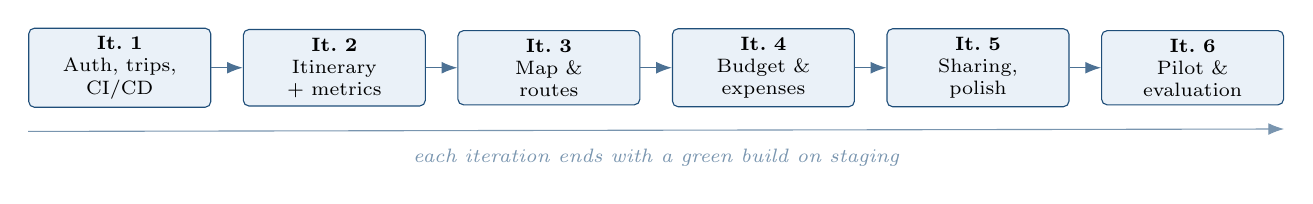
\begin{tikzpicture}[
  ph/.style={draw=teAccent,fill=teFill,rounded corners=2pt,
    align=center,font=\scriptsize,minimum height=9mm,text width=21mm,inner sep=3pt},
  ar/.style={-{Latex[length=2mm]},draw=teAccent!80}
]
\node[ph] (p1) {\textbf{It.\ 1}\\Auth, trips,\\CI/CD};
\node[ph,right=4mm of p1] (p2) {\textbf{It.\ 2}\\Itinerary\\+ metrics};
\node[ph,right=4mm of p2] (p3) {\textbf{It.\ 3}\\Map \&\\routes};
\node[ph,right=4mm of p3] (p4) {\textbf{It.\ 4}\\Budget \&\\expenses};
\node[ph,right=4mm of p4] (p5) {\textbf{It.\ 5}\\Sharing,\\polish};
\node[ph,right=4mm of p5] (p6) {\textbf{It.\ 6}\\Pilot \&\\evaluation};
\foreach \a/\b in {p1/p2,p2/p3,p3/p4,p4/p5,p5/p6} \draw[ar] (\a)--(\b);
\draw[teAccent!60,-{Latex[length=2mm]}] ($(p1.south west)+(0,-3mm)$) -- ($(p6.south east)+(0,-3mm)$)
  node[midway,below=1.2mm,font=\scriptsize\itshape] {each iteration ends with a green build on staging};
\end{tikzpicture}
\caption{Illustrative iteration roadmap.}
\label{fig:roadmap}
\end{figure}

\subsection{Out of scope for this course}
Weather, AI-generated itineraries, collaborative
real-time editing, hotel and transport booking, and
multi-language support are recorded as future scope.
Listing them here is a scope boundary, not a promise.

\section{Risks and mitigations}
\begin{itemize}[leftmargin=0.7cm]
    \item \textbf{Maps quota and billing.} Autocomplete
      is the expensive call. Mitigation: debounce
      input, use session tokens, cap per-user calls in
      development, and keep the itinerary usable
      without the map so a quota exhaustion degrades
      one feature instead of the product.
    \item \textbf{Key exposure.} A committed or
      unrestricted key is the realistic security
      failure for a project of this kind. Mitigation:
      keys in environment variables only; the browser
      key restricted by HTTP referrer and by API; the
      Directions key used only from server-side route
      handlers; a secret scan in CI.
    \item \textbf{Authorisation defects.} With no
      server tier, Firestore rules \emph{are} the
      authorisation layer. Mitigation: rules are
      version-controlled and unit-tested against the
      emulator in CI; the default is deny.
    \item \textbf{Scope creep towards AI features.}
      Mitigation: the out-of-scope list above is
      treated as binding for the course; anything on it
      needs an explicit decision to move.
    \item \textbf{Vendor lock-in.} Mitigation: all data
      access goes through service modules rather than
      being called from components, so the surface that
      would have to change is small and enumerable.
    \item \textbf{Uneven contribution across three
      members.} Mitigation: work tracked as issues with
      named owners, review required before merge, and
      the per-member journals in this repository as the
      record.
\end{itemize}

\section{Summary}
TripEase proposes a web application that keeps a
trip's itinerary, geography and budget in one shared
record, addressing workflow fragmentation rather than
any absence of tools. It fits the course criteria on
each heuristic: the stakeholders are our immediate
peers and the problem is observable now; every
component is a mature, documented engine, with the one
genuinely hard sub-problem deliberately reduced to an
overridable heuristic; the architecture is deployable
on managed services from iteration~1; and success is
defined by a measurable, system-attributable metric
--- time-to-complete-itinerary against an observed
baseline --- fixed in advance.

Nothing described here has been implemented yet. This
document is a proposal, and the numbers in \S6 are
targets to be tested, not findings.

\end{document}
